\section{Results}
Firstly in figure \ref{robotProgress} we can see the progress a robot (R) has made towards the target (E). 

\begin{figure}
	\centering
	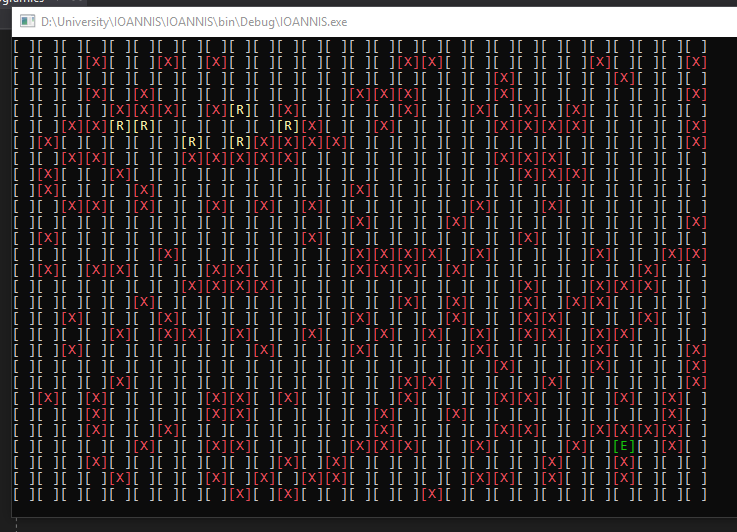
\includegraphics[width=0.9\linewidth]{ui}
	\caption{Initial robot progress.}
	\label{robotProgress}
\end{figure}

The Rs clustered in the upper right hand corner represent each of the robots trying to find their way to the objective.

We can then see more progress having been made in figure \ref{morerobotProgress}. This demonstrates how much improvement can be made over a short number of generations.
\begin{figure}
	\centering
	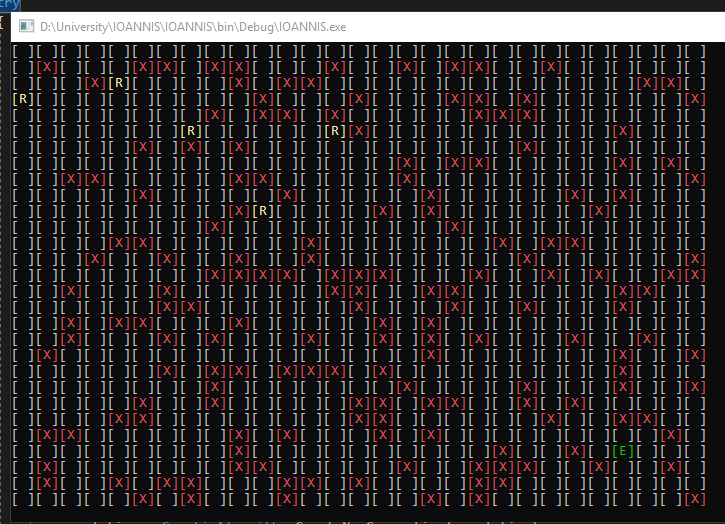
\includegraphics[width=0.9\linewidth]{moreProgress}
	\caption{Robot progress at generation 4.}
	\label{morerobotProgress}
\end{figure}

While initially the behaviour may seem random, over generations will start to follow a similar trend.

\begin{figure}
	\centering
	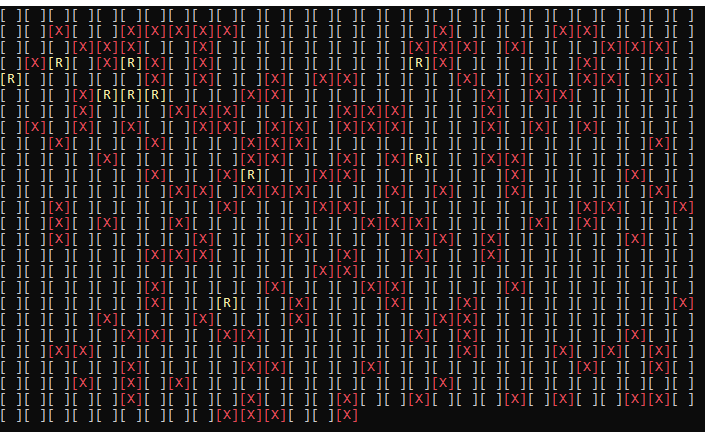
\includegraphics[width=0.9\linewidth]{evenMoreProgress}
	\caption{Continued evolution.}
	\label{evenmorerobotProgress}
\end{figure}
Then in figure \ref{evenmorerobotProgress} we can see that progress can continue even further. 

\begin{figure}
	\centering
	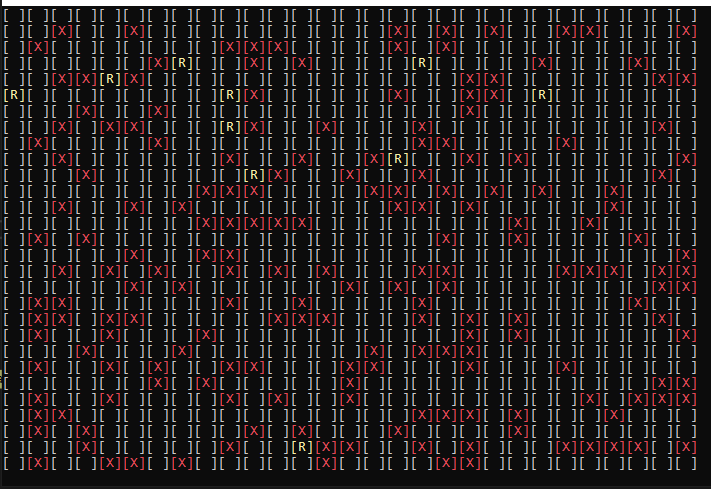
\includegraphics[width=0.9\linewidth]{somuchProgress}
	\caption{Generation 21 flag capture.}
	\label{evenmorerobotProgress}
\end{figure}
Lastly \ref{somuchProgress} Shows a robot having successfully captured the flag at the bottom of the image at generation 21. 

\subsection{Evaluation}

This project has shown that with enough time a robot is able to complete it's objective in relatively few generations - 21. This has given us useful knowledge to be applied to future research. This has also shown that with even more attention to the fitness function, even better results can be achieved. However, that said, as can be seen by figure \ref{evenmorerobotProgress}. With the correct ammount of time, this algorithm definitely shows improvement.